\documentclass[../PaulGanssle-Thesis.tex]{subfiles}

\begin{document}
\chapter{Blueprints}
% An appendix dedicated to blueprints of various components of the magnetometers, labeled with scales
\label{blueprints}
Many of the components of the magnetometer have been designed and re-designed during the process of development of a practical device for NMR measurements. This appendix collects each of these designs for all components of the magnetometer to document these changes and give a more exact sense of the instrumentation used in these experiments. Strictly speaking, these are technical drawings produced by AutoCAD, and are not produced by blue-printing, a process wherein technical drawings are copied by the application of a light to the originals, which sit on top of a paper coated in a ferro-gallate solution. The ferro-gallate solution is light-sensitive, and where no lines are present exposure causes the ferro-gallate to convert into a stable blue dye. With the advent of digital home printing, this process is no longer necessary, and the word ``blueprint'' is merely a skeuomorph from a bygone age.

\begin{figure}[p]
\centering
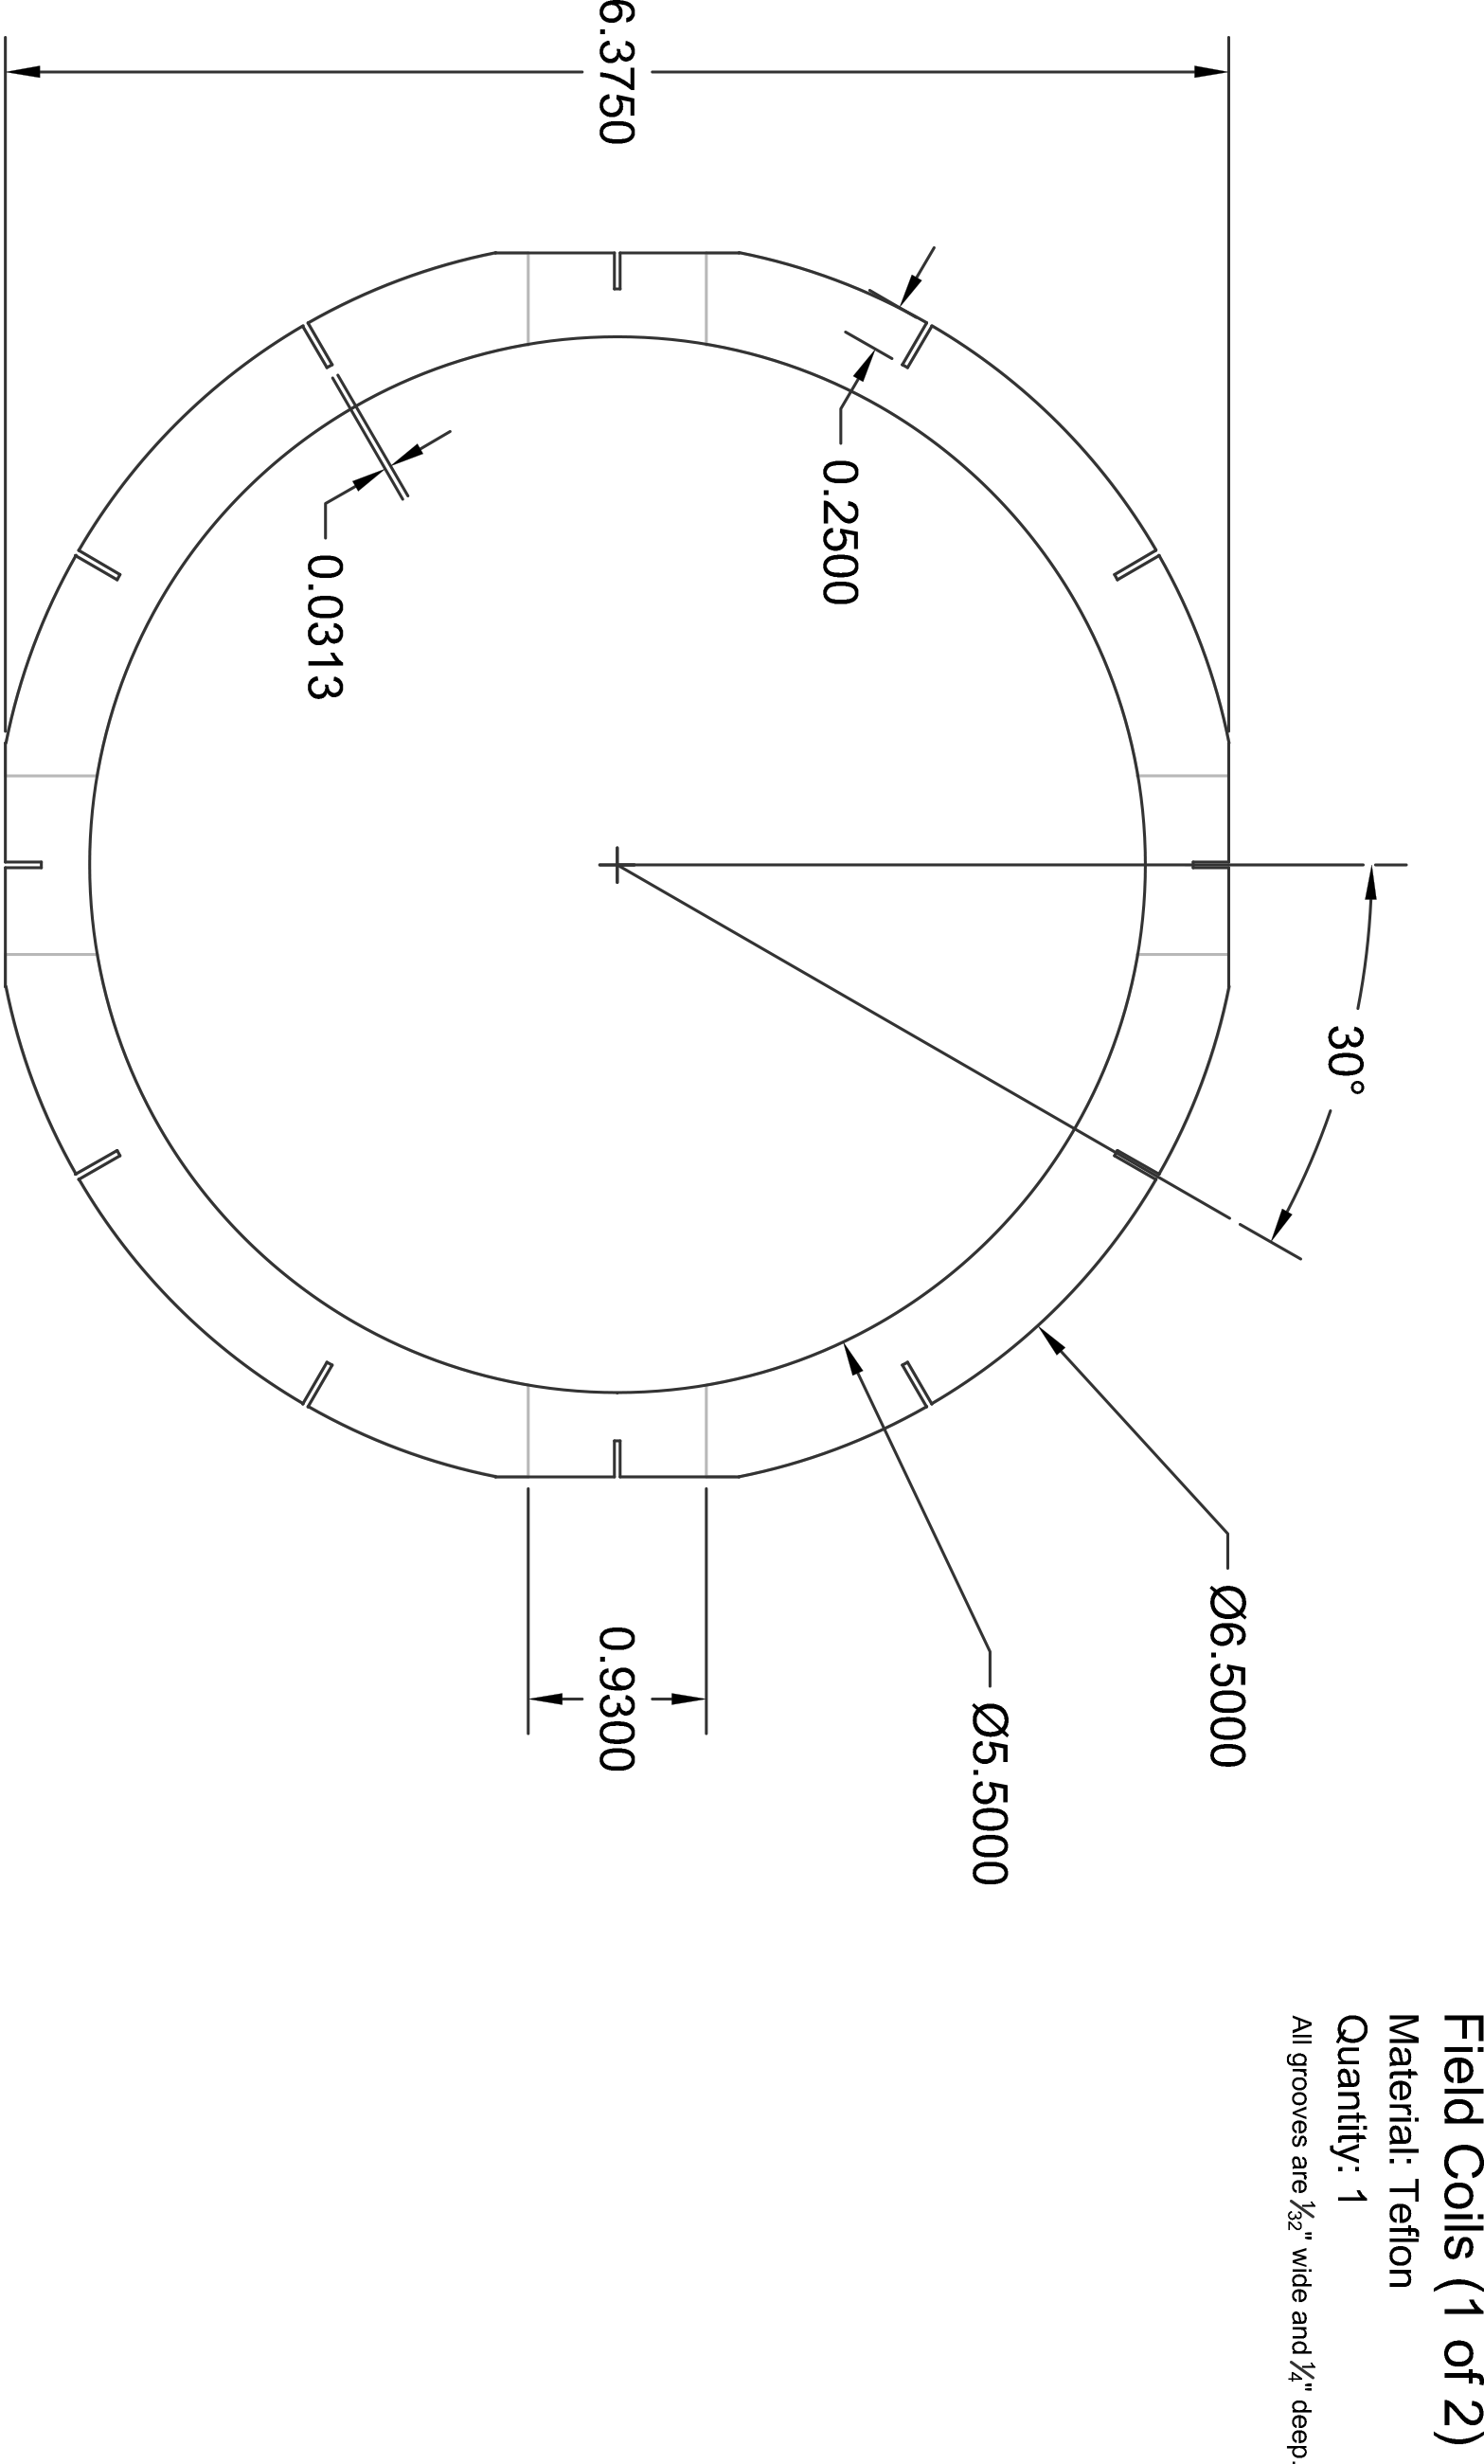
\includegraphics[height=0.95\textheight]{appendices/blueprints/ShimCoils01-Radial.png}
\caption{The shim field coil substrate, radial (top) view.}
\label{blueprints:FieldCoils-Radial}
\end{figure}

\begin{figure}[p]
\centering
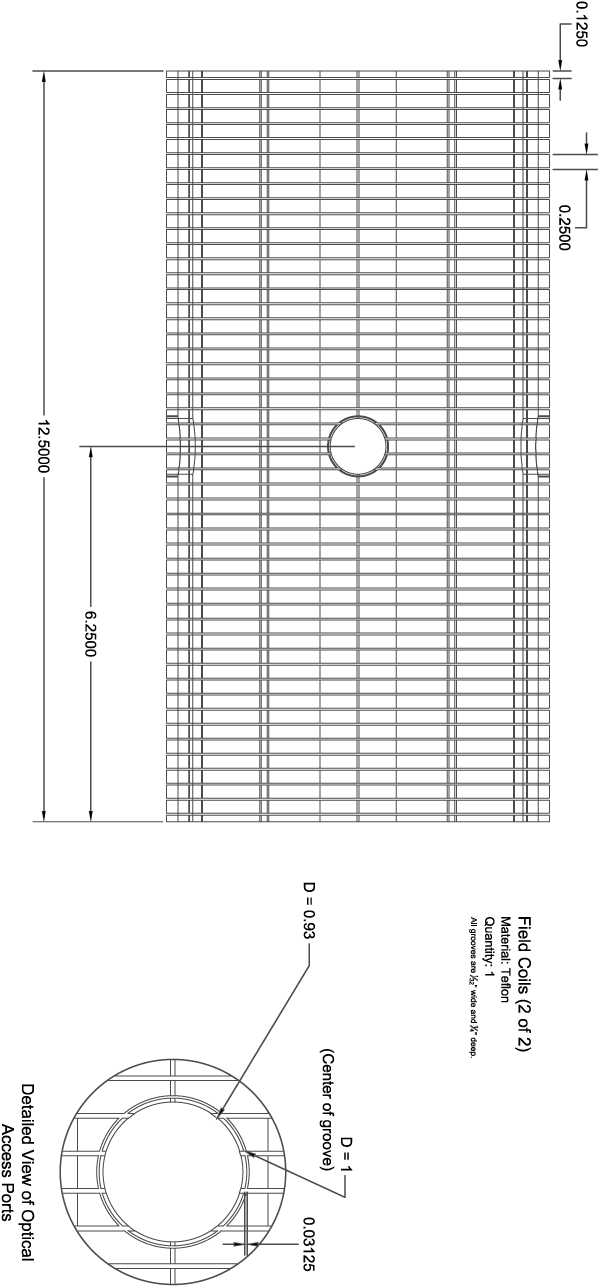
\includegraphics[height=0.95\textheight]{appendices/blueprints/ShimCoils02-Side.png}
\caption{The shim field coil substrate, side view.}
\label{blueprints:FieldCoils-Side}
\end{figure}

\begin{figure}[p]
\centering
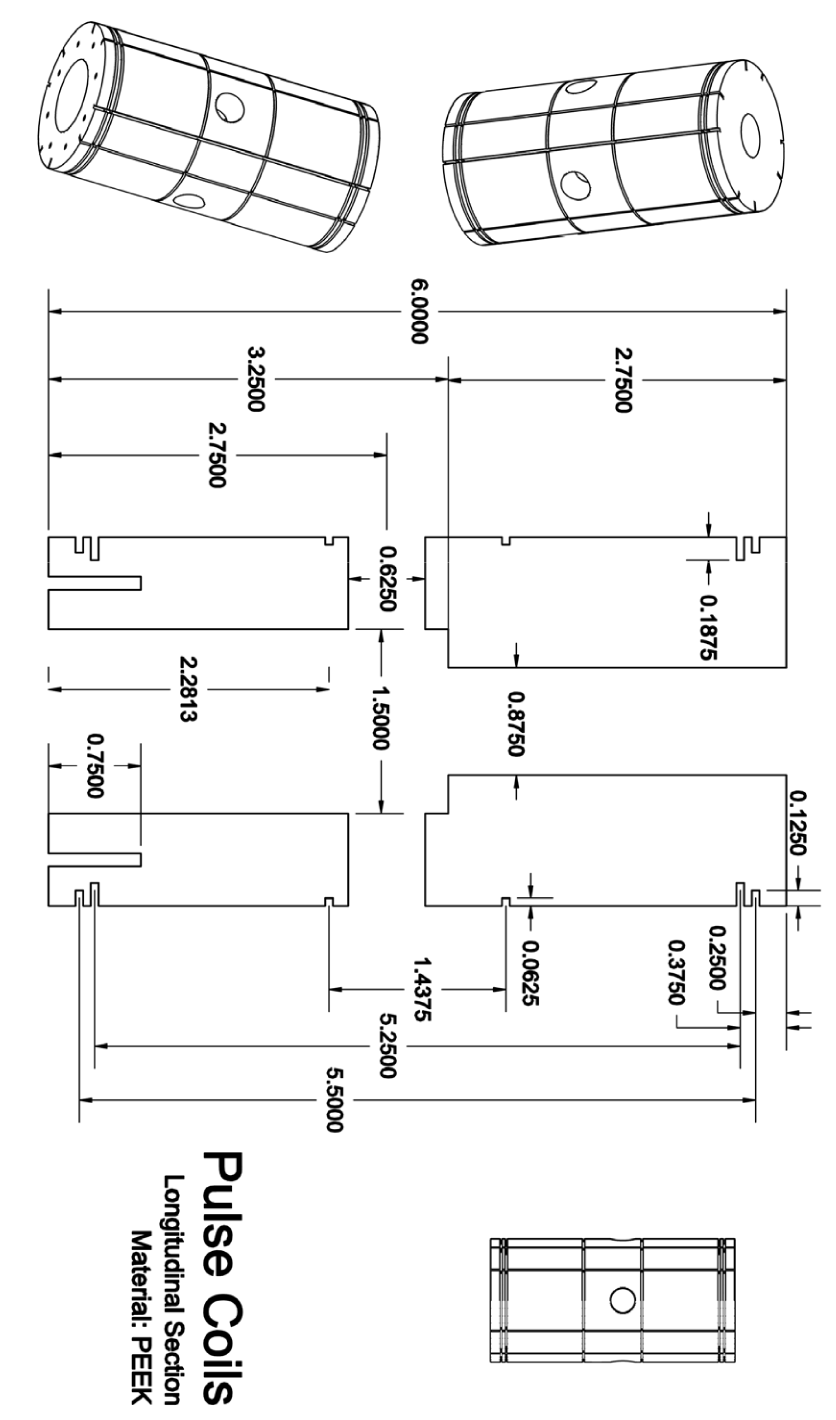
\includegraphics[height=0.95\textheight]{appendices/blueprints/PulseCoils01.png}
\caption{The new, more homogeneous pulse coils, longitudinal (side) view.}
\label{blueprints:NewPulseCoils01}

\end{figure}
\begin{figure}[p]
\centering

\includegraphics[height=0.95\textheight]{appendices/blueprints/PulseCoils02.png}
\caption{The new, more homogeneous pulse coils, transverse (top) view.}
\label{blueprints:NewPulseCoils02}
\end{figure}

\begin{figure}[p]
\centering
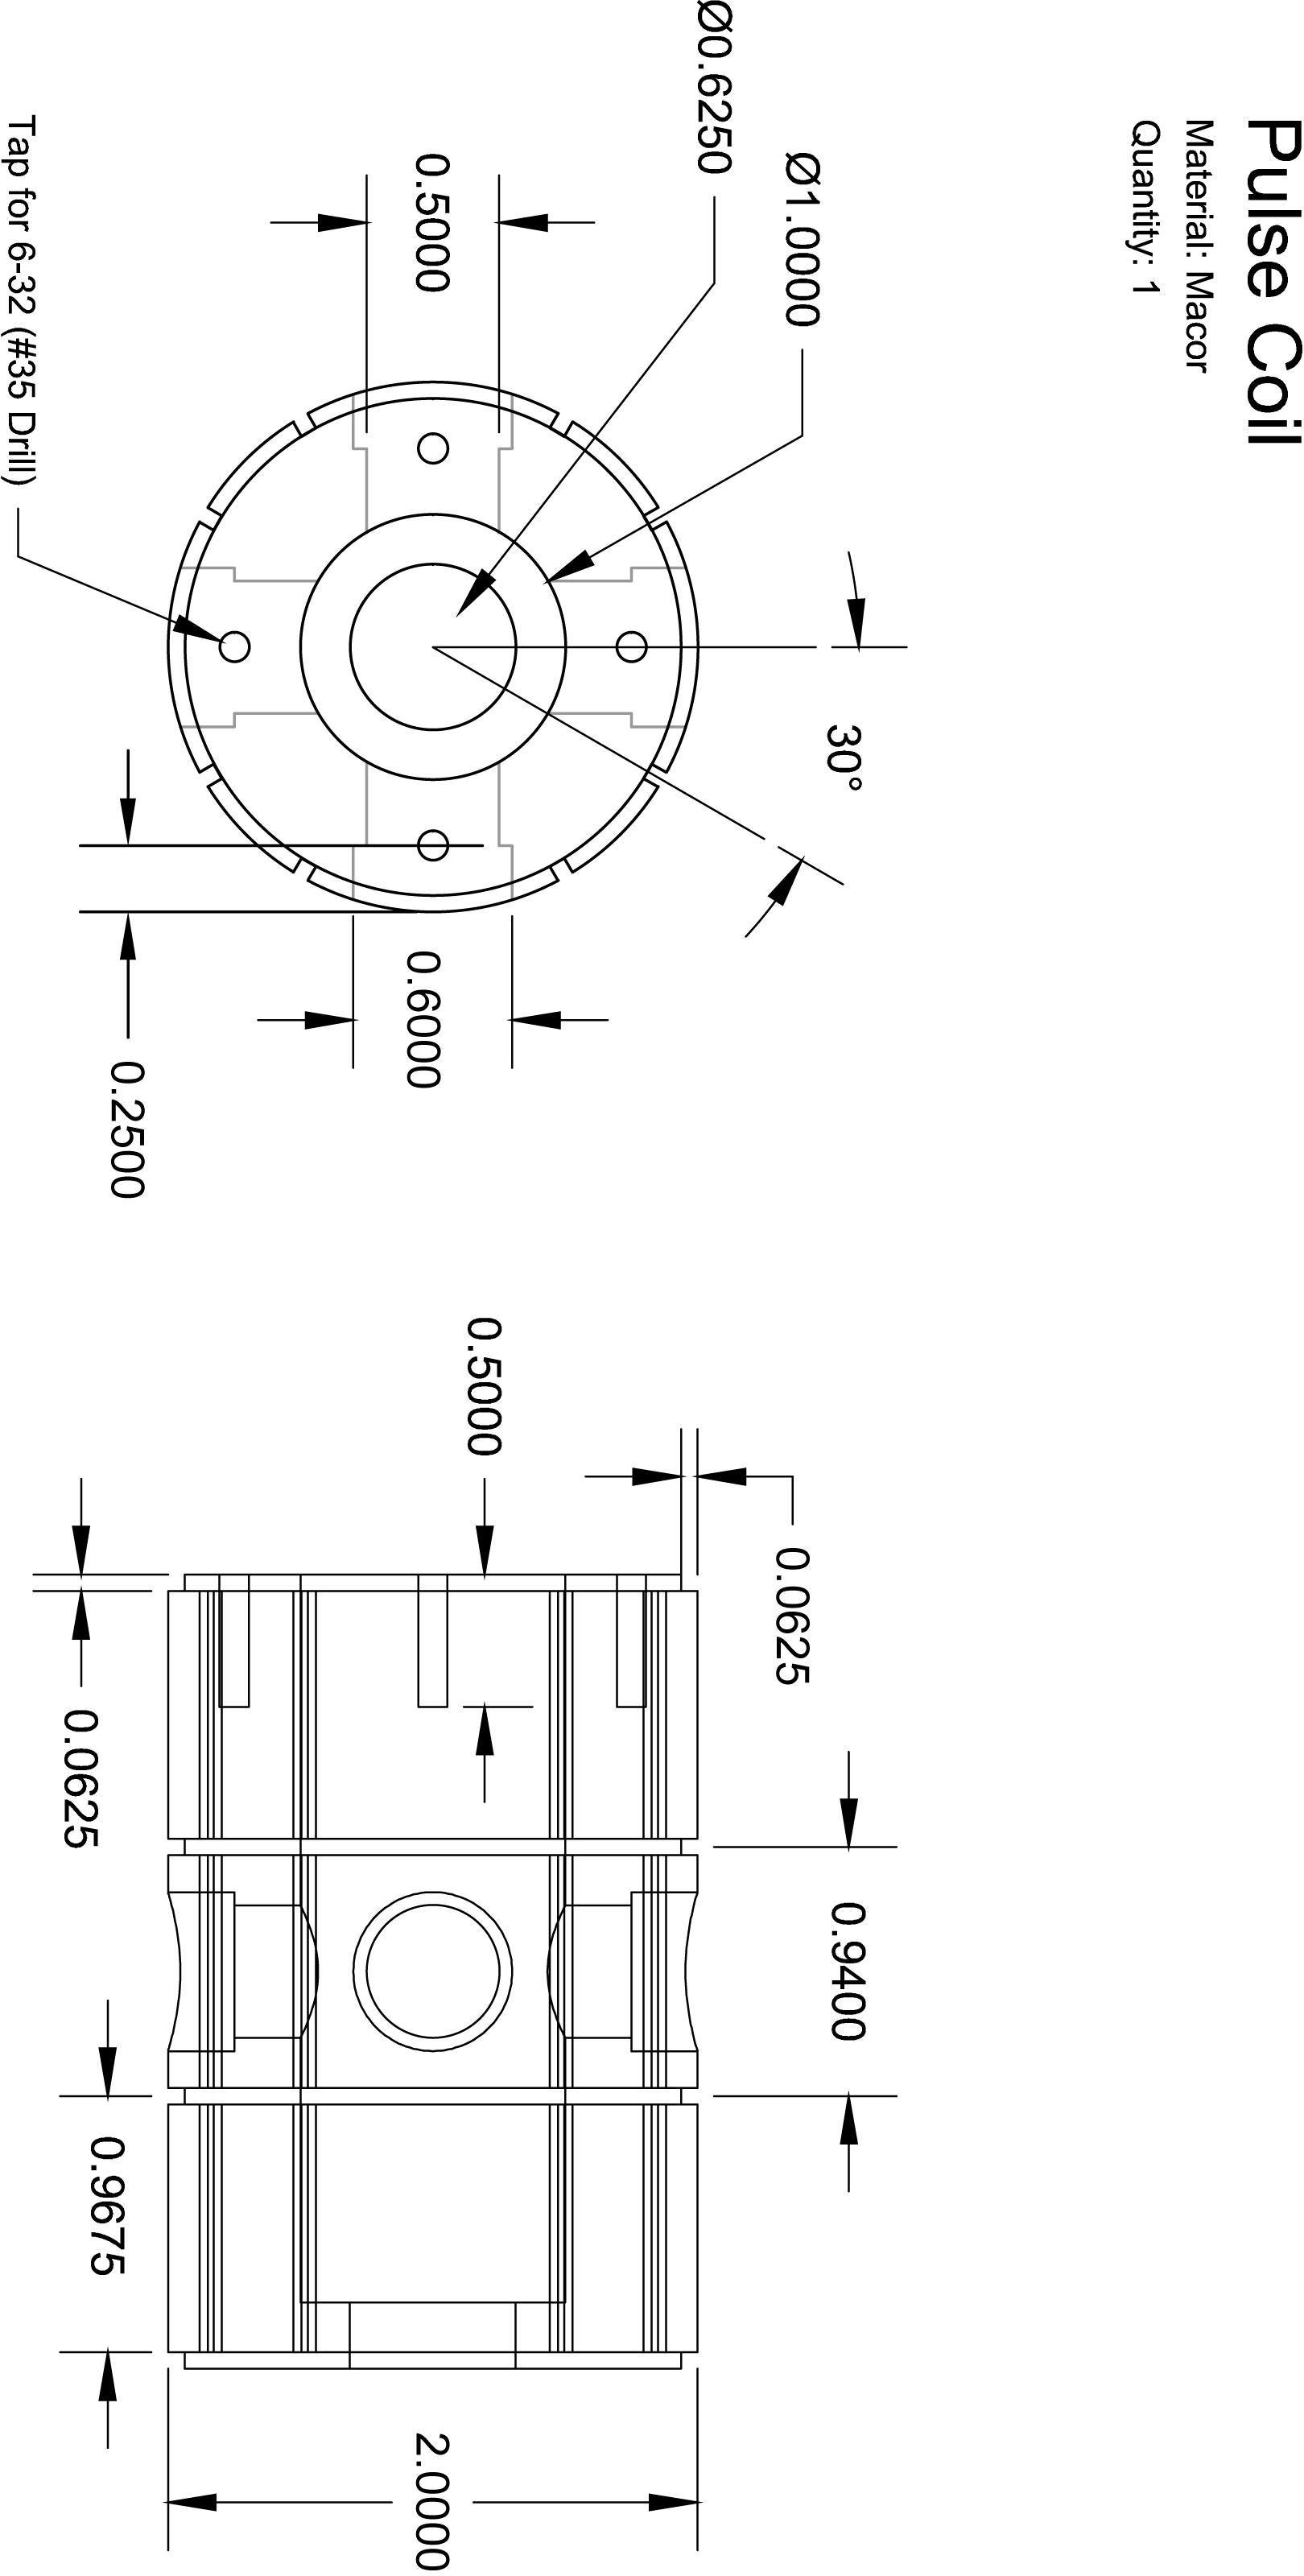
\includegraphics[height=0.95\textheight]{appendices/blueprints/OldPulseCoils.png}
\caption{The older, inhomogeneous pulse coils.}
\label{blueprints:OldPulseCoils}
\end{figure}

\begin{figure}[p]
\centering
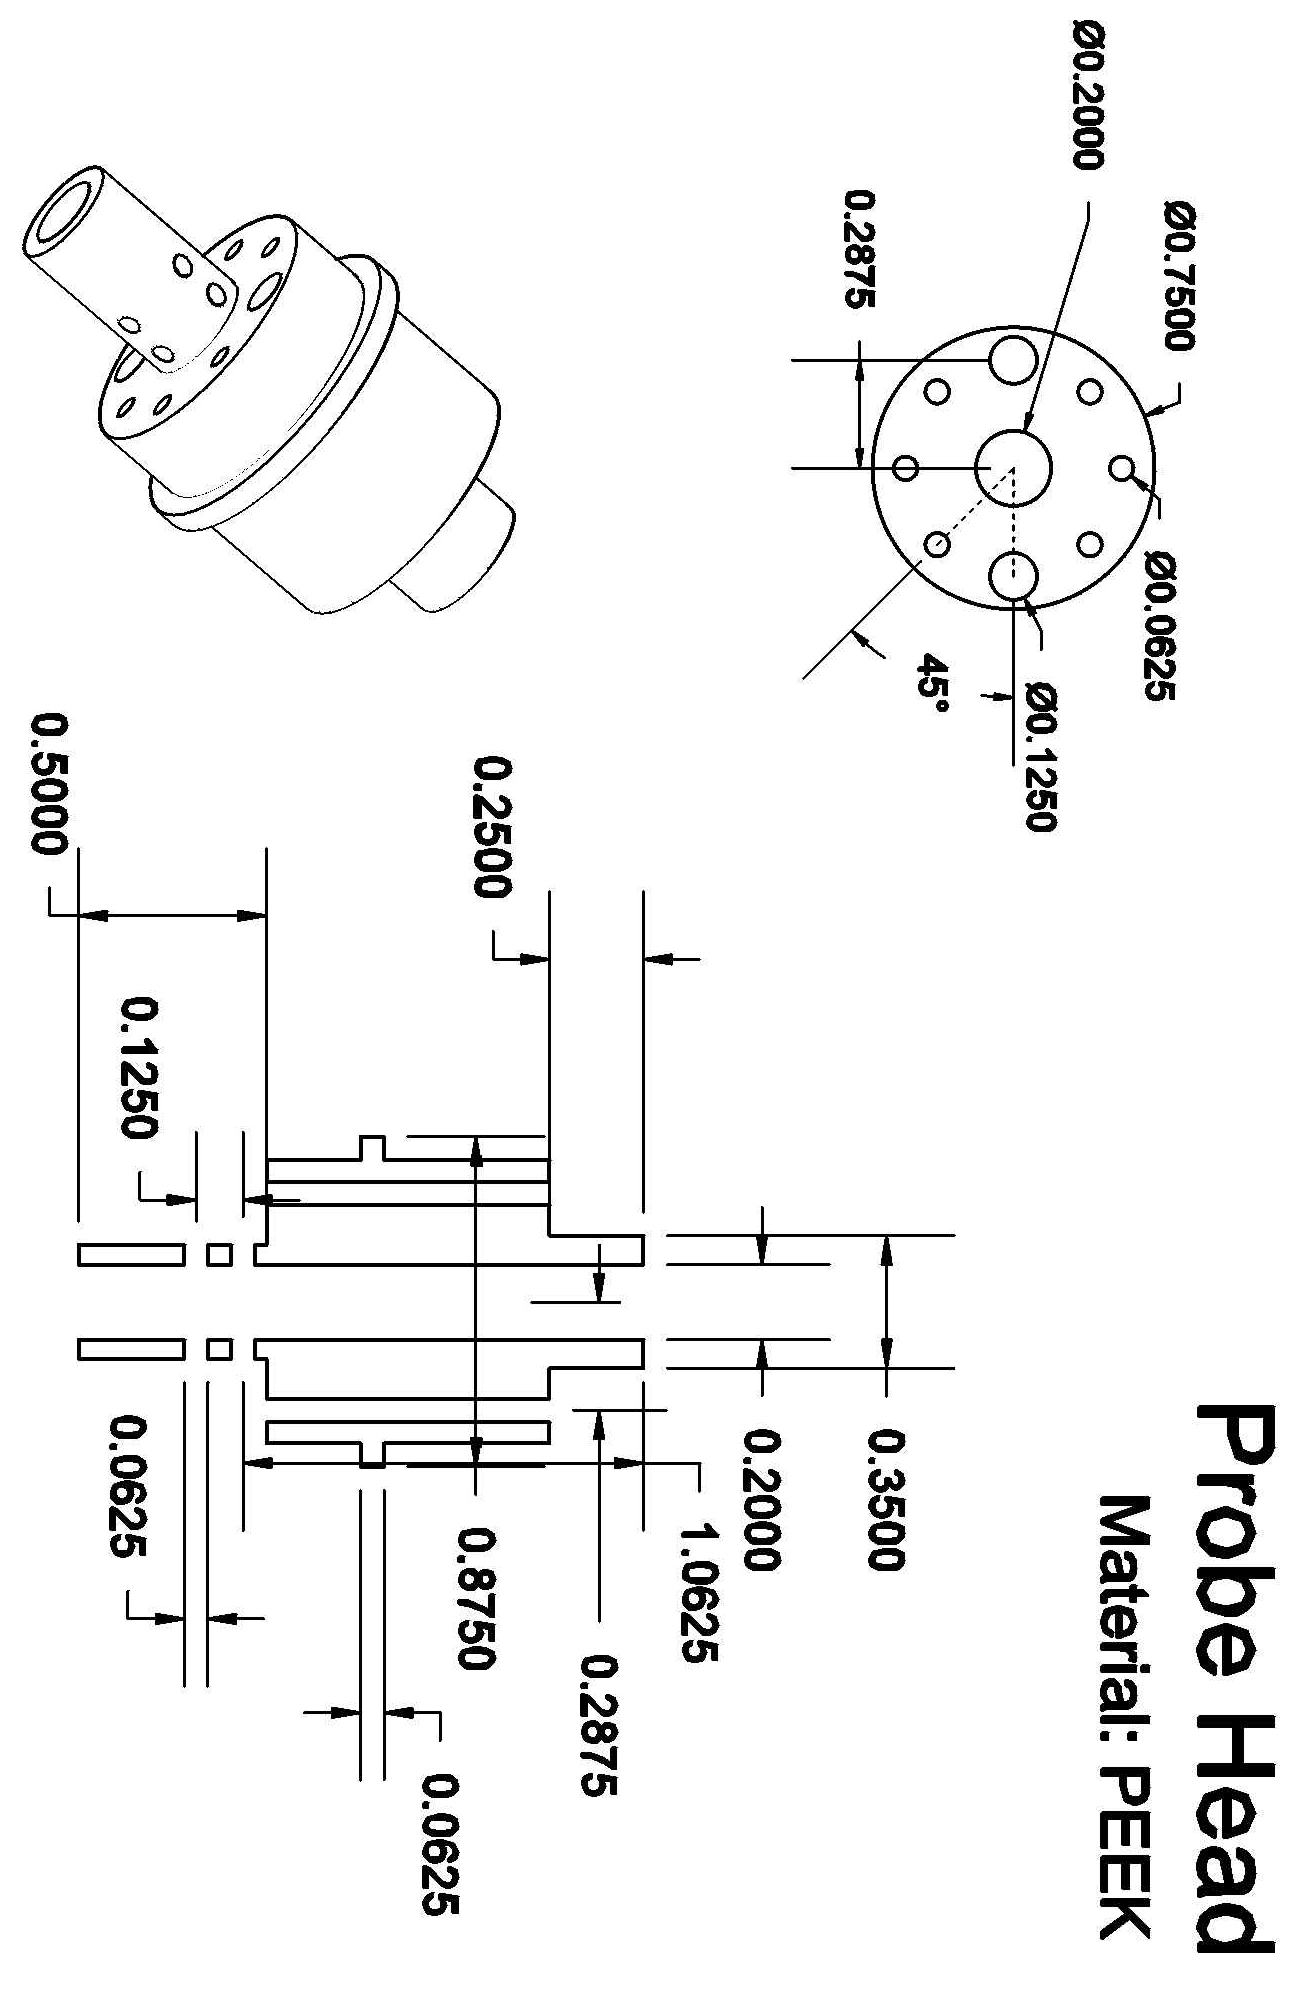
\includegraphics[height=0.95\textheight]{appendices/blueprints/ProbeHead.png}
\caption{The probe head body.}
\label{blueprints:ProbeHead}
\end{figure}

\begin{figure}[p]
\centering
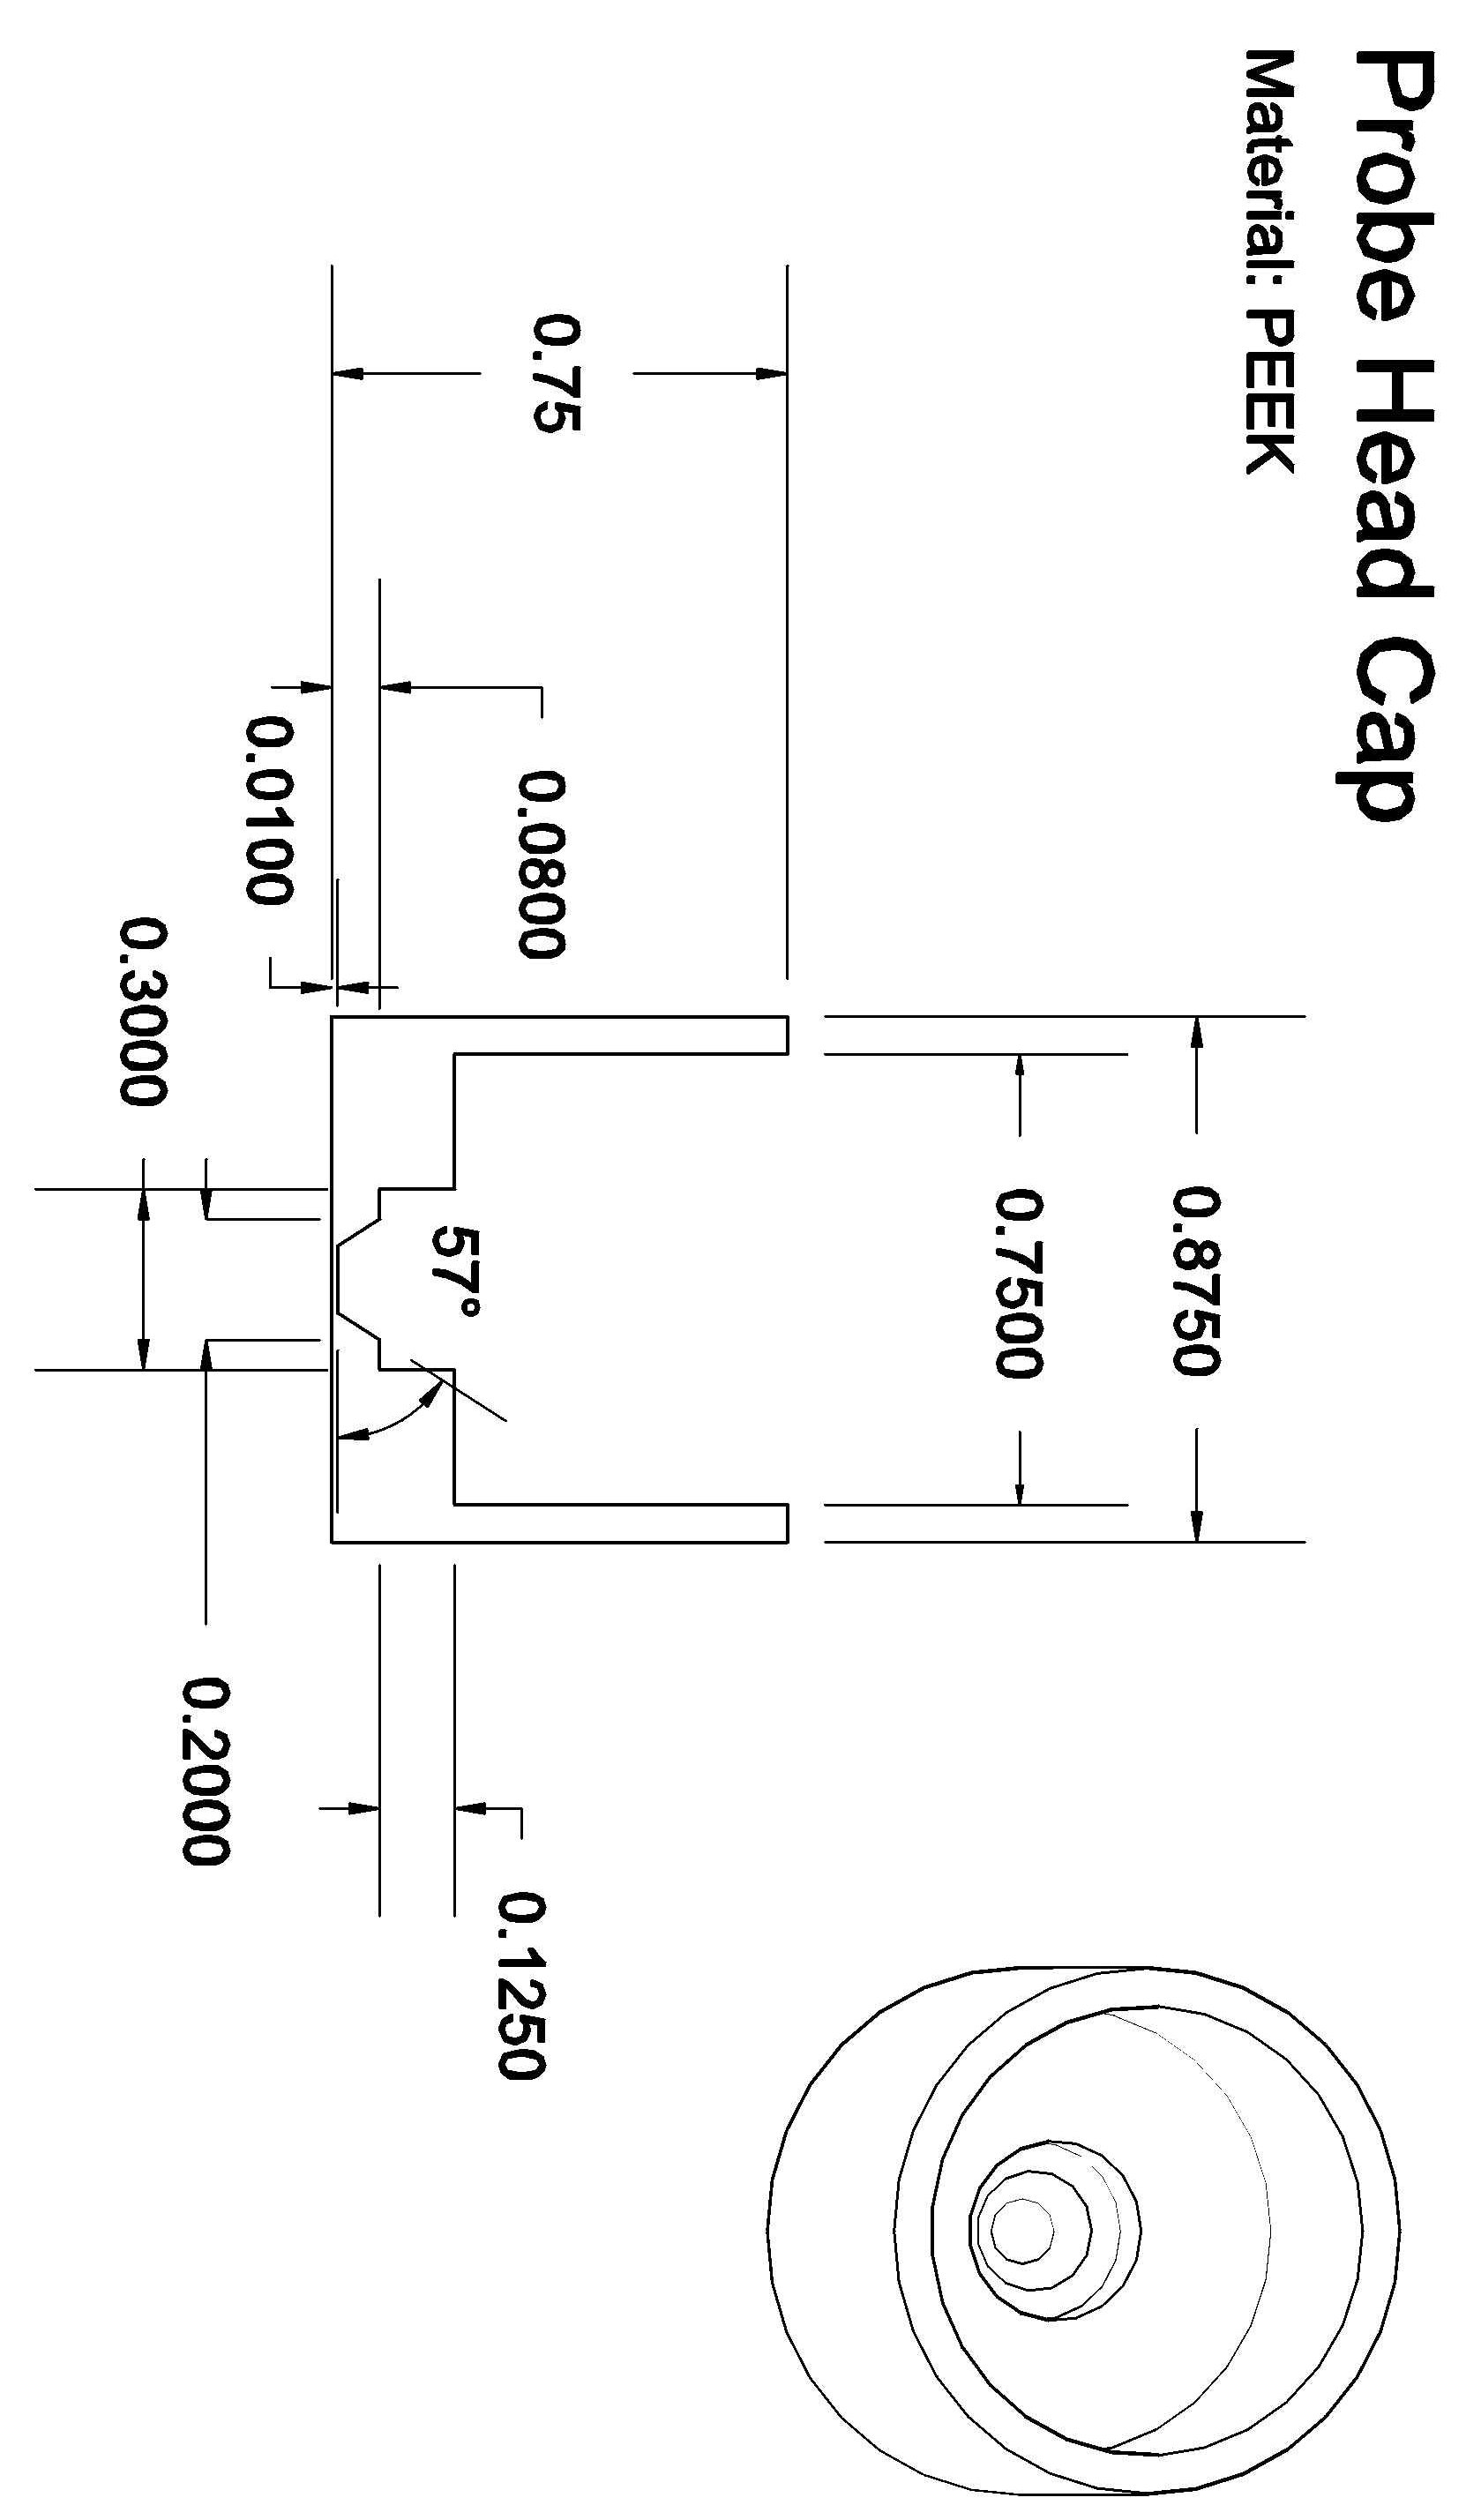
\includegraphics[height=0.95\textheight]{appendices/blueprints/ProbeHeadCap.png}
\caption{The probe head cap.}
\label{blueprints:ProbeHeadCap}
\end{figure}

\end{document}
